\subsection{The Current Conveyor}

\subsubsection{Introduction}

In voltage-mode circuits, the main building block used to add, subtract, amplify, attenuate, and filter voltage signals is the operational amplifier. In current-mode circuits, the analogous building block is the \textit{current conveyor}. It really came from a need of an op-amp for the current mode function - which is funny because the idea of current conveyor was invented before the circuit was invented ( discovered/engineered or whatever you may want to call it). 

\begin{figure}[H]
    \centering
    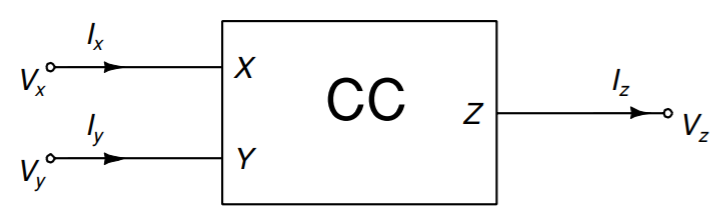
\includegraphics[width=0.8\linewidth]{../../Figures/Current_Conveyor.PNG}
    \caption{The current conveyor. Adapted from Textbook.}
    \label{fig:Current_Conveyor}
\end{figure}

If we want to do current mode computation, we need a building block that that can convey current from input terminl to output terminl while \textit{decoulpling} the circuit, just like an op-amp where $V_1$ and $V_2$ are the input which come with infinite impedance, and then you have the output $V_{out}$ - so you completely decouple the input from the output. We need the same in current mode. We also want to use this builidng block to do basic computations (add, multiply, filter etc...). Here is the formal definition: 

\begin{itemize}
    \item The potential at the output terminal (Z) is independant of the current applied at node Y
    \item An input current that is forced into node X results in an equal amount of current flowing into node Y.
    \item The input current flowing into node X is conveyed to node Z, which has the characteristics of a high output impedance current source.
\end{itemize}

\begin{figure}[H]
    \centering
    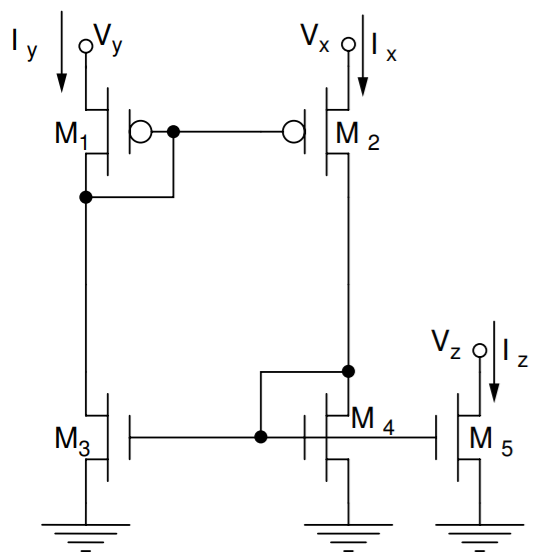
\includegraphics[width=0.8\linewidth]{../../Figures/Current_Conveyor_Circuit.PNG}
    \caption{A circuit which satisfies that the current conveyor definition. Adapted from Lecture notes.}
    \label{fig:Current_Conveyor_Circuit}
\end{figure}

Briefly looking at Figure \ref{fig:Current_Conveyor_Ciruit}, which is a potential current mirror, the input terminals are $X$ and $Y$, the output is at $Z$. If you apply a current through $Y$, it results in the same current through $X$ because of the current mirror, which is copied again at $M3$ and $M4$ which yields that whatever flows through Y is conveyed to Z. Again this is just one example of a current conveyor, which actually is just unity in this circuit. 

\subsubsection{Basic subthreshold current conveyor}

Figure \ref{fig:Current_Conveyor_Ciruit_2} shows a current conveyor that is commonly used at the institute of Neuroinformatics, and the one we should know about. 

\begin{figure}[H]
    \centering
    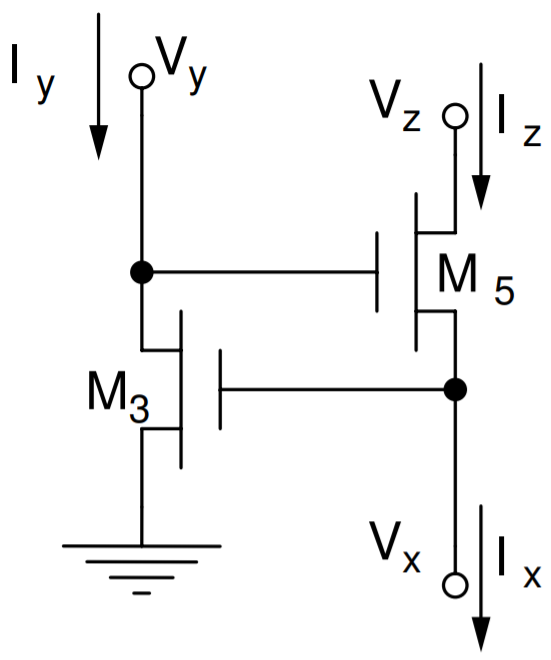
\includegraphics[width=0.8\linewidth]{../../Figures/Current_Conveyor_Circuit_2.PNG}
    \caption{A common current conveyor circuit. This is the one you should know for the exam. Adapted from Lecture notes.}
    \label{fig:Current_Conveyor_Circuit_2}
\end{figure}

Here we force a current into node $V_y$ which is copied into node $V_x$. How does that work? Let's go through it: 
\begin{itemize}
    \item If you \textit{force} the current $I_y$ through $M_3$, the gate voltage of $M_3$ \textit{must adapt} to the log of the current flowing through it \footnote{because (omitting $\kappa, I_0$ and $U_T$ for simplicity: $I = exp(V_{gs}) so V_{gs} = log(I)$)}.  So $V_x \propto \mathrm{ln}(I_y)$.
    \item Now we set $I_x$ (which is another input of the circuit) to be equal to $I_y$ (or proportionality factor of $I_y$, we will exactly like before force the $V_{gs} = V_y - V_x$ of $M_5$ to follow log$(I_x)$. 
    \item This then results into $I_z$ whic must follow $I_x$
    \item So to summarize, two take aways about this: 1) $I_z = I_x$ and 2) $V_x \propto \mathrm{ln}(I_y)$
    \item It decouples input current from output current. 
\end{itemize}

It's used in a broad range of circuits such as: 
\begin{itemize}
    \item Low pass filters
    \item Multiplier circuits 
    \item Winner take all circuits 
    \item Silicon Neurons
    \item Current-mode silicon retinas
\end{itemize}